\section{Snapshots}

A snapshot stores the state of a virtual machine at a specific point in time. This allows you to revert to that state, should you need to. Unlike backups which store the entire state of the virtual machine, snapshots only store the changes made since the snapshot was taken.
\\\\
The snapshot feature is very similar in Proxmox and vSphere. Both support making extensive snapshot trees, where you can have snapshots of a snapshot of a snapshot including different branches. You can choose whether to also snapshot the memory state of the VM or not. In Proxmox the VM disk must either be stored as qcow2 image available to file level storage, or on a storage type that supports snapshots. For a complete list see~\ref{tab:storageTable}.
\\\\
Here is an example of a snapshot tree in Proxmox, the VM is currently running under the state of test1, but I could always revert back to test2 through test4.

\begin{figure}[H]
	\centering
	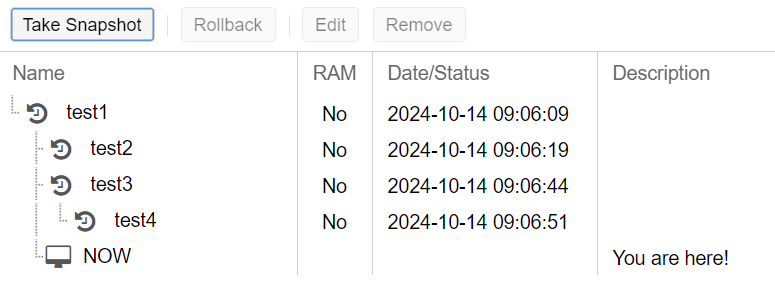
\includegraphics[width=0.8\linewidth]{Proxmox_snapshots.png} % Figure image
	\caption{Snapshot tree in Proxmox} % Figure caption
	\label{fig:Snapshot tree in Proxmox} % Label for referencing with \ref{bear}
\end{figure}